%% This Beamer template is based on the one found here: https://github.com/sanhacheong/stanford-beamer-presentation, and edited to be used for Stanford ARM Lab

\documentclass[10pt]{beamer}
%\mode<presentation>{}

\usepackage{media9}
\usepackage{amssymb,amsmath,amsthm,enumerate}
\usepackage{mathtools}
\usepackage[utf8]{inputenc}
\usepackage{array}
\usepackage[parfill]{parskip}
\usepackage[utf8]{vietnam}
\usepackage{graphicx,animate}
\usepackage{caption}
\usepackage{subcaption}
\usepackage{bm}
\usepackage{amsfonts,amscd}
\usepackage[]{units}
\usepackage{listings}
\usepackage{multicol}
\usepackage{multirow}
\usepackage{tcolorbox}
\usepackage{physics}
\usepackage{movie15}
% Enable colored hyperlinks
\hypersetup{colorlinks=true}

% The following three lines are for crossmarks & checkmarks
\usepackage{pifont}% http://ctan.org/pkg/pifont
\newcommand{\cmark}{\ding{51}}%
\newcommand{\xmark}{\ding{55}}%

% Numbered captions of tables, pictures, etc.
\setbeamertemplate{caption}[numbered]
\usepackage{media9} 
%\usepackage[superscript,biblabel]{cite}
%\usepackage{algorithmic}
%\usepackage{algorithm2e}
\usepackage{algpseudocode}
%\usepackage[linesnumbered,ruled,vlined]{algorithm2e}
\usepackage{algorithm}
%\usepackage{algorithmic}
\usepackage{caption}
%\usepackage{xcolor}
\usepackage{array}
%\renewcommand{\thealgocf}{}

\usepackage[natbib,backend=biber,style=ieee, sorting=ynt]{biblatex}
\bibliography{ref.bib}

\usepackage[acronym]{glossaries}

\usepackage{graphicx}
\graphicspath{{./figures}}
\usepackage{hyperref}

\theoremstyle{remark}
\newtheorem*{remark}{Remark}
\theoremstyle{definition}

\newcommand{\empy}[1]{{\color{darkorange}\emph{#1}}}
\newcommand{\empr}[1]{{\color{cardinalred}\emph{#1}}}
\newcommand{\examplebox}[2]{
\begin{tcolorbox}[colframe=darkcardinal,colback=boxgray,title=#1]
#2
\end{tcolorbox}}

\usetheme{Stanford} 
\def \i  {\item}
\def \ai {\item[] \quad \arrowbullet}
\newcommand \si[1]{\item[] \quad \bulletcolor{#1}}
\def \wi {\item[] \quad $\ \phantom{\Rightarrow}\ $}
\def \bi {\begin{itemize}\item}
\def \ei {\end{itemize}}
\def \be {\begin{equation*}}
\def \ee {\end{equation*}}
\def \bie {$\displaystyle{}
\def \eie {{\ }$}}
\def \bsie {\small$\displaystyle{}
\def \esie {{\ }$}\normalsize\selectfont}
\def \bse {\small\begin{equation*}}
\def \ese {\end{equation*}\normalsize}
\def \bfe {\footnotesize\begin{equation*}}
\def \efe {\end{equation*}\normalsize}
\renewcommand \le[1] {\\ \medskip \lefteqn{\hspace{1cm}#1} \medskip}
\def \bex {\begin{example}}
\def \eex {\end{example}}
\def \bfig {\begin{figure}}
\def \efig {\end{figure}}
\def \btheo {\begin{theorem}}
\def \etheo {\end{theorem}}
\def \bc {\begin{columns}}
\def \ec {\end{columns}}
\def \btab {\begin{tabbing}}
\def \etab {\end{tabbing}\svneg\svneg}
\newcommand \col[1]{\column{#1\linewidth}}
\def\vneg  {\vspace{-5mm}}
\def\lvneg {\vspace{-10mm}}
\def\svneg {\vspace{-2mm}}
\def\tvneg {\vspace{-1mm}}
\def\vpos  {\vspace{5mm}}
\def\lvpos {\vspace{10mm}}
\def\svpos {\vspace{2mm}}
\def\tvpos {\vspace{1mm}}
\def\hneg  {\hspace{-5mm}}
\def\lhneg {\hspace{-10mm}}
\def\shneg {\hspace{-2mm}}
\def\thneg {\hspace{-1mm}}
\def\hpos  {\hspace{5mm}}
\def\lhpos {\hspace{10mm}}
\def\shpos {\hspace{2mm}}

\logo{
\includegraphics[height=0.5in]{logos/HUS-name.jpg}}

\makeatletter
\let\@@magyar@captionfix\relax
\makeatother

\title[Tối ưu hóa nâng cao]{Tối ưu hóa nâng cao: Bài tập 3}

\begin{document}

\nocite{*}

\author[Nguyễn Chí Thanh - Nguyễn Đức Thịnh]{
	\begin{tabular}{c} 
	\Large
	Nguyễn Chí Thanh \\
    \footnotesize \href{mailto:nguyenchithanh\_sdh21@hus.edu.vn}{nguyenchithanh\_sdh21@hus.edu.vn} \\
	\Large
    Nguyễn Đức Thịnh \\
     \footnotesize \href{mailto:nguyenducthinh\_sdh21@hus.edu.vn}{nguyenducthinh\_sdh21@hus.edu.vn}
\end{tabular}
\vspace{-4ex}}

\institute{
	\vskip 5pt
	\begin{figure}
		\centering
		\begin{subfigure}[t]{0.5\textwidth}
			\centering
			
\includegraphics[height=0.75in]{logos/HUS-logo.jpg}
		\end{subfigure}%
		~ 
		\begin{subfigure}[t]{0.5\textwidth}
			\centering
			
\includegraphics[height=0.75in]{logos/MIM-logo.png}
		\end{subfigure}
	\end{figure}
	\vskip 10pt	
	Đại học Quốc Gia Hà Nội \\
	Trường đại học Khoa học tự nhiên\\
	Khoa Toán - Cơ - Tin học
	\vskip 3pt
}

\begin{noheadline}
\begin{frame} \maketitle \end{frame}
\end{noheadline}
    
\setbeamertemplate{itemize items}[default]
\setbeamertemplate{itemize subitem}[circle]

\begin{frame}{Nội dung}

    \begin{enumerate}
		\item Bài toán hồi quy tuyến tính
        \item So sánh ba thuật toán
        \item So sánh nhiều thuật toán
        \item Kết luận
    \end{enumerate}
    
\end{frame}

\begin{frame}[allowframebreaks]{Bài toán hồi quy tuyến tính}
	\begin{itemize}
		\item Hàm loss của Linear Regression:
		\begin{equation*}
			f(w) = \lVert X w - y \rVert_2^2
		\end{equation*}
		\item Ta đặt kích thước các ma trận $X \in \mathbb{R}^{m \times n}, y \in \mathbb{R}^m, w \in \mathbb{R}^n$, ta có $\mathrm{dom}(f)=\mathbb{R}^{n}$ là tập lồi
		\begin{equation*}
			\begin{aligned}
				f(w) &= (Xw - y)^T (Xw - y) \\
				&=w^T X^T X w - w^TX^Ty - y^T Xw + y^T y
			\end{aligned}
		\end{equation*}
		\item Do $w^TX^Ty$ và $y^TXw$ là hai số vô hướng và $(w^TX^Ty)^T=y^TXw$ nên $w^TX^Ty=y^TXw$ (chuyển vị của một số vô hướng bằng chính nó) nên:
		\begin{equation*}
			\begin{aligned}
				f(w) &= w^T X^T X w - w^TX^Ty - y^T Xw + y^T y\\
				&=w^T X^T X w-2w^TX^Ty+y^Ty
			\end{aligned}
		\end{equation*}
		\item Ta tính Gradient của $f(w)$ theo $w$:
		\begin{equation*}
			\nabla f(w) =\Big\lbrack X^TX + (X^TX)^T \Big\rbrack w - 2X^Ty = 2X^T X w - 2 X^T y
		\end{equation*}
		\item Ta tính ma trận Hessian của $f(w)$ theo $w$:
		\begin{equation*}
			\nabla^2 f(w) = 2X^T X
		\end{equation*}
		\item Ta xét:
		\begin{equation*}
			p^T \nabla^2 f(w) p = 2 p^T X^T X p = 2 (Xp)^TXp \geq 0 \thickspace\forall \thickspace p \in \mathbb{R}^{n}
		\end{equation*}
		nên:
		\begin{equation*}
			\nabla^2 f(w) \succeq 0 \thickspace \forall w \in \mathbb{R}^{n}
		\end{equation*}
		\item Vì $\mathrm{dom}(f)$ là tập lồi và $\nabla^2 f(w) \succeq 0$ nên hàm $f(w)$ là một hàm lồi.
	\end{itemize}
	Hàm loss được sử dụng trong lập trình:
	\begin{equation*}
		f(w) = \dfrac{1}{n}\sum_{i=1}^{n}\Big( x_i^T w - y_i \Big)^2
	\end{equation*}
	với $(x_i, y_i) \in \mathbb{R}^{n+1}, i=1, 2, \dots, n$ là cặp dữ liệu đầu vào và nhãn tương ứng với $w \in \mathbb{R}^n$
	
	\framebreak
	Nghiệm tối ưu (khi các cột của ma trận $X$ độc lập tuyến tính):

	\begin{equation*}
		w^{*} = \Big(X^T X \Big)^{-1}X^T y
	\end{equation*}

	Với dữ liệu tập train:

	\begin{equation*}
		w_{train}^{*} = \begin{bmatrix} -1.3962 &  0.3796 & 0.5107 & -0.04332 &\\ 0.07553 & 0.5786 & 0.1703 & 0.07757 &\\ 1.2154  & 1.2375 &  0.8117  & 0.16389 &\\ -0.5221 &  0.4350 & -0.0788 & -0.5564 \end{bmatrix}
	\end{equation*}

	và giá trị hàm loss tương ứng:

	\begin{equation*}
		f(w_{train}^{*}, \text{ data }_{\text{train}}) \approx 0.04804
	\end{equation*}

	\begin{equation*}
		f(w_{train}^{*}, \text{ data }_{\text{val}}) \approx 0.04959
	\end{equation*}

	\framebreak
	
	Với dữ liệu tập validation:

	\begin{equation*}
		\centering
		w_{val}^{*} = \begin{bmatrix} -0.8715 &  0.2894 & -2.0394 & 0.08472 &\\ 0.04182 &  0.6075 & 0.1884 &  0.05182 &\\ 1.1757 &   2.07476 &    1.6335  & 0.04724 & \\ -0.3275 & 0.4018 & -0.0500 & -0.5091  \end{bmatrix}
	\end{equation*}

	và giá trị hàm loss tương ứng:

	\begin{equation*}
		f(w_{val}^{*}, \text{ data }_{\text{train}}) \approx 0.06977
	\end{equation*}

	\begin{equation*}
		f(w_{val}^{*}, \text{ data }_{\text{val}}) \approx 0.06900
	\end{equation*}
\end{frame}

\begin{frame}{So sánh nhiều thuật toán}
	Các thuật toán được so sánh:
	\begin{multicols}{3}
	\begin{enumerate}
		\item Gradient Descent
  		\item Newton
    	\item Accelerated
     	\item BFGS
      	\item DFP
        \item Momentum
        \item Adagrad
        \item Adadelta
        \item RMSProp
        \item Adam
        \item Adamax
        \item AMSGrad
        \item Nadam
        \item AdaBelief
        \item RAdam
        \item Avagrad    
	\end{enumerate}
	\end{multicols}
	Các step size: $10^{-4}, 10^{-3}, 10^{-2}, 10^{-1}, 1, 2, 5, 10$
	
	Các kiểu chọn step size từng bước: Fixed, Backtracking, Inverse decay, Warmup, Triangular Cyclic

\end{frame}
	%\begin{figure}
	%	\centering
	%	\begin{subfigure}[b]{0.45\textwidth}
	%		\centering
	%		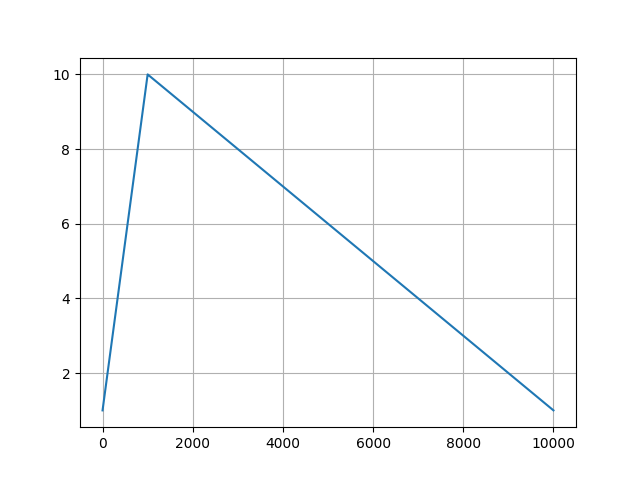
\includegraphics[width=\textwidth]{Thanh/warmup_lr.png}
	%		\caption{$y=x$}
	%	\end{subfigure}
	%	\hfill
	%	\begin{subfigure}[b]{0.45\textwidth}
	%		\centering
	%		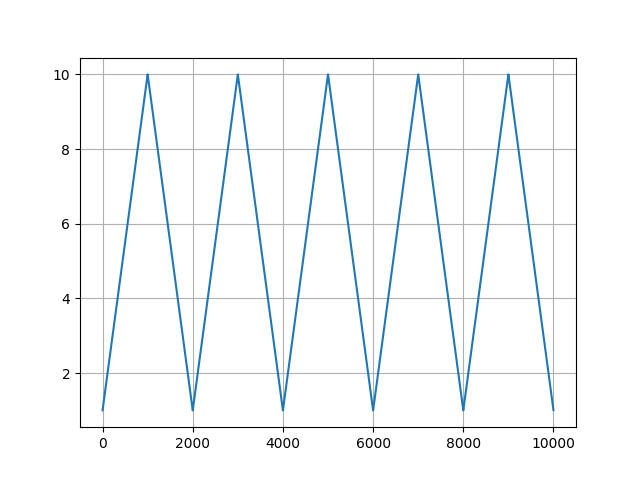
\includegraphics[width=\textwidth]{Thanh/triangular_cyclic.png}
	%		\caption{$y=3sinx$}
	%	\end{subfigure}
	%\end{figure}

\begin{frame}{So sánh nhiều thuật toán}
	\begin{figure}[!htp]
		% Maximum length
		\subfloat[Warmup step size]{\label{fig1:a}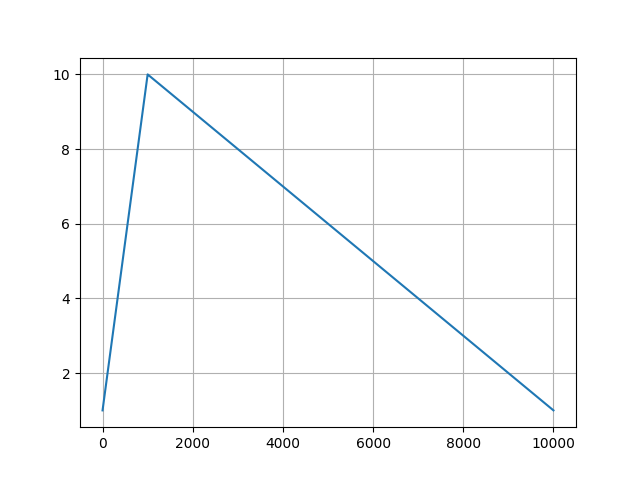
\includegraphics[width=0.5\linewidth]{Thanh/warmup_lr.png}}\hfill
		\subfloat[Triangular cyclic step size]{\label{fig1:b}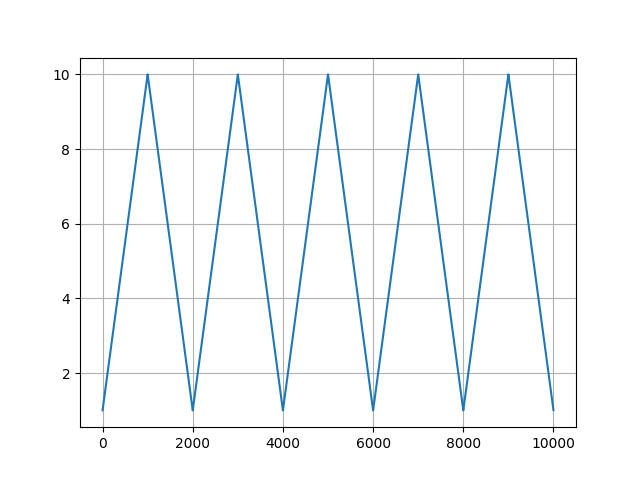
\includegraphics[width=0.5\linewidth]{Thanh/triangular_cyclic.png}}%
	  \end{figure}

	Mỗi nhóm gồm thuật toán tối ưu, step size, kiểu chọn step size sẽ tạo thành một tổ hợp.
	Một tổ hợp được dùng để train 5000 bước

\end{frame}

\begin{frame}[allowframebreaks]{So sánh nhiều thuật toán}
	\framesubtitle{Các hình vẽ so sánh với trục hoành là số bước}
	\begin{figure}
		\centering
		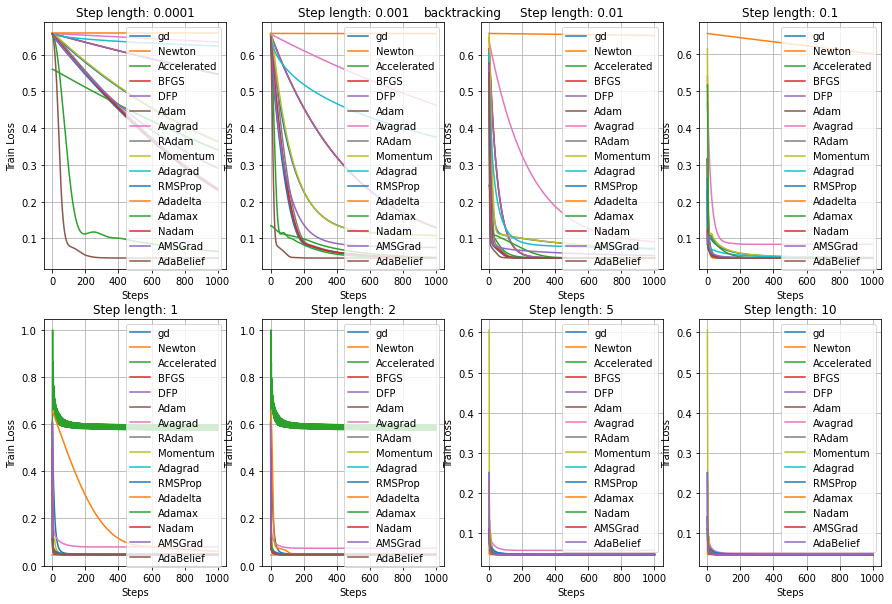
\includegraphics[width=10cm]{Thanh/backtrack-lr-step-op_step.png}
		\caption{So sánh các thuật toán với phương pháp backtracking tìm step size}
	\end{figure}

	\begin{figure}
		\centering
		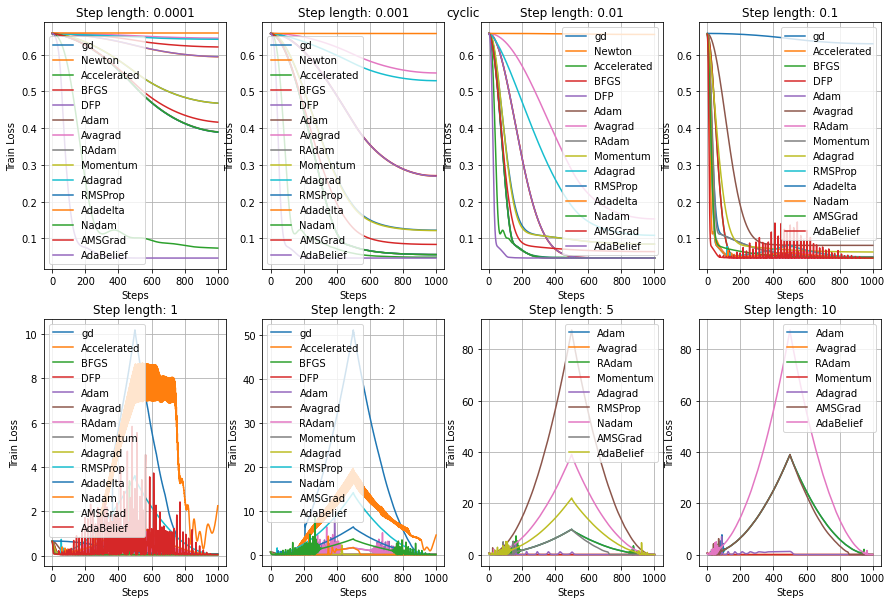
\includegraphics[width=10cm]{Thanh/cyclic-lr-step-op_step.png}
		\caption{So sánh các thuật toán với phương pháp cyclic}
	\end{figure}

	\begin{figure}
		\centering
		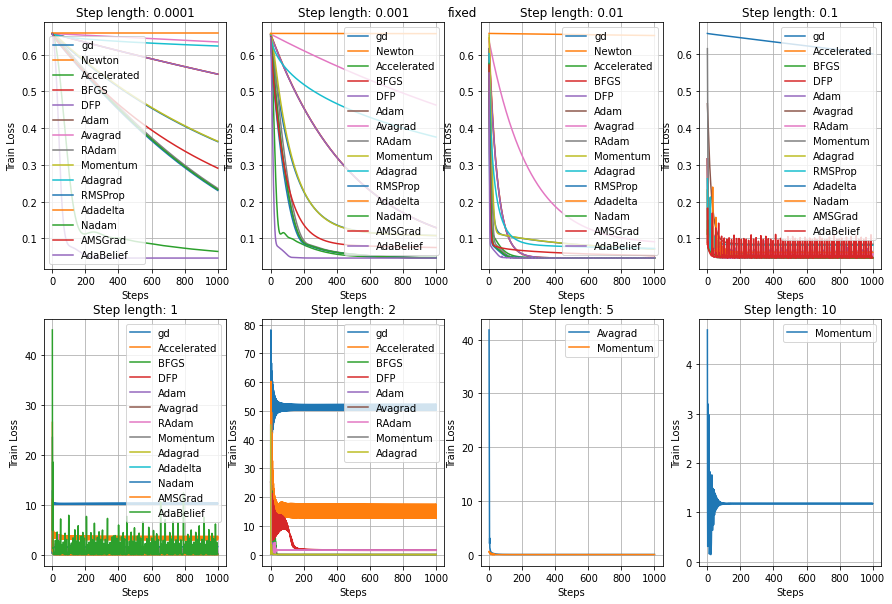
\includegraphics[width=10cm]{Thanh/fixed-lr-step-op_step.png}
		\caption{So sánh các thuật toán với phương pháp cố định step size}
	\end{figure}

	\begin{figure}
		\centering
		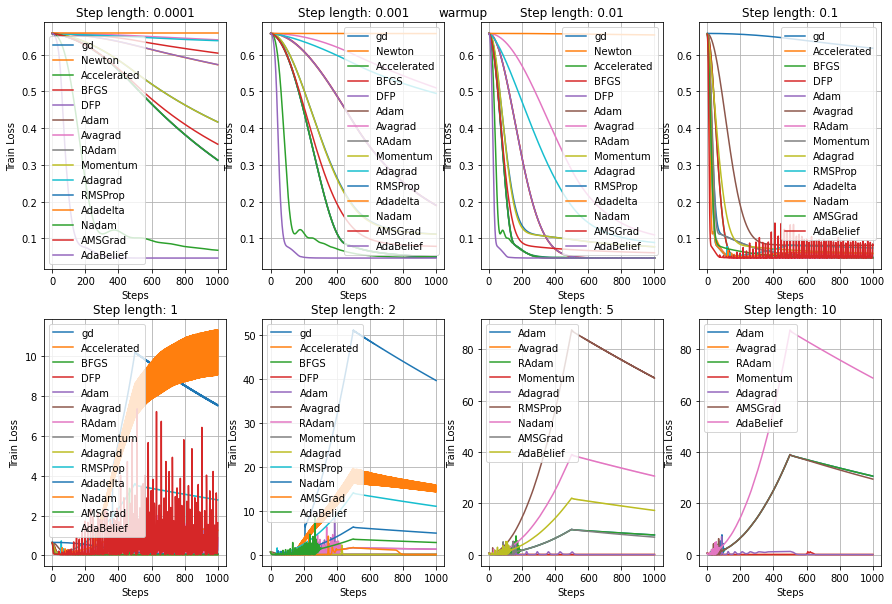
\includegraphics[width=10cm]{Thanh/warmup-lr-step-op_step.png}
		\caption{So sánh các thuật toán với phương pháp warmup step size}
	\end{figure}

	\begin{figure}
		\centering
		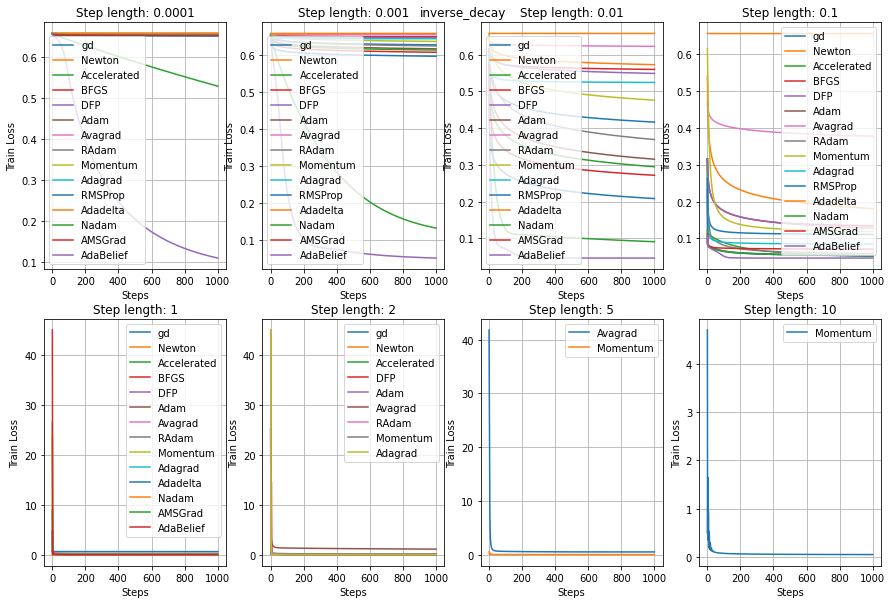
\includegraphics[width=10cm]{Thanh/inverse-lr-step-op_step.png}
		\caption{So sánh các thuật toán với phương pháp giảm step size dạng hyperbol}
	\end{figure}
\end{frame}


\begin{frame}[allowframebreaks]{So sánh nhiều thuật toán}
	\framesubtitle{Các hình vẽ so sánh với trục hoành là thời gian (giây)}
	\begin{figure}
		\centering
		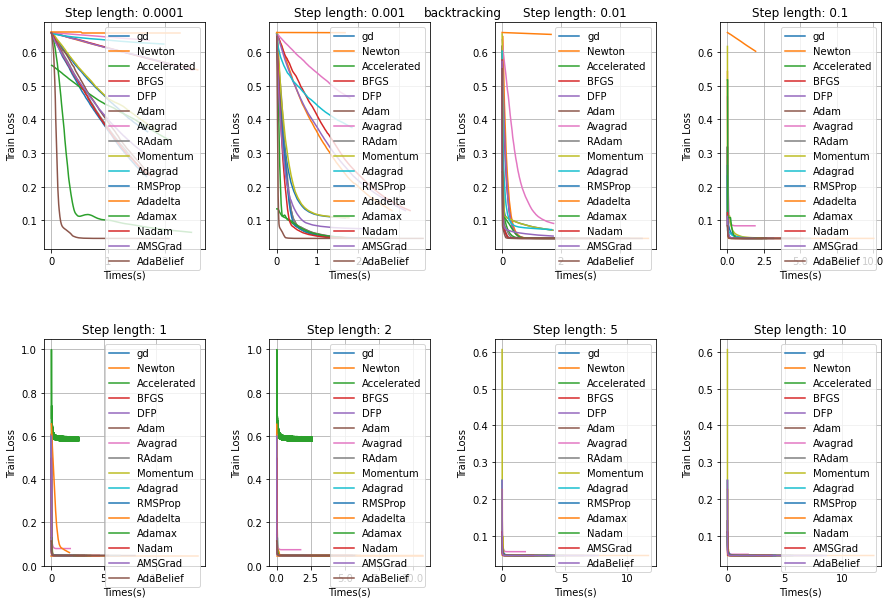
\includegraphics[width=10cm]{Thanh/backtrack-lr-step-op_time.png}
		\caption{So sánh các thuật toán với phương pháp backtracking tìm step size}
	\end{figure}

	\begin{figure}
		\centering
		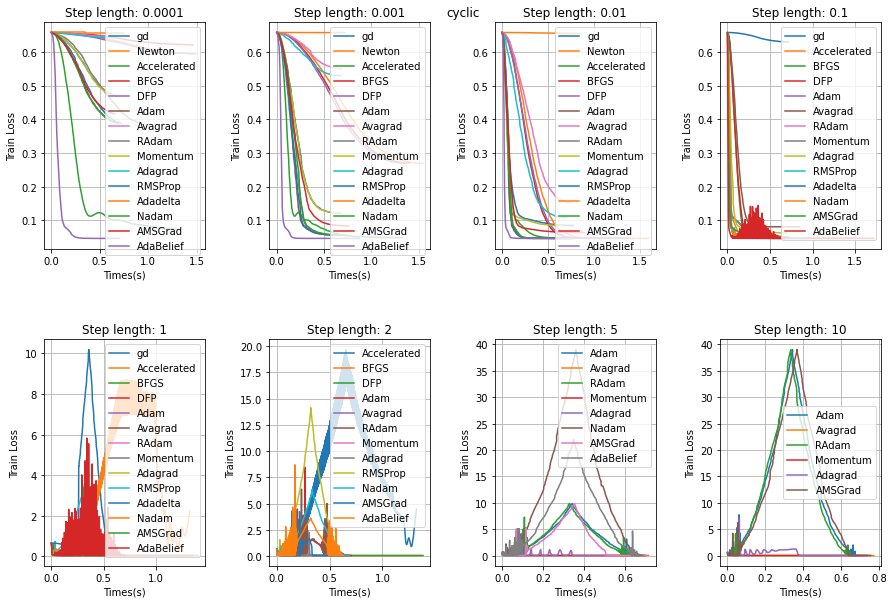
\includegraphics[width=10cm]{Thanh/cyclic-lr-step-op_time.png}
		\caption{So sánh các thuật toán với phương pháp cyclic}
	\end{figure}

	\begin{figure}
		\centering
		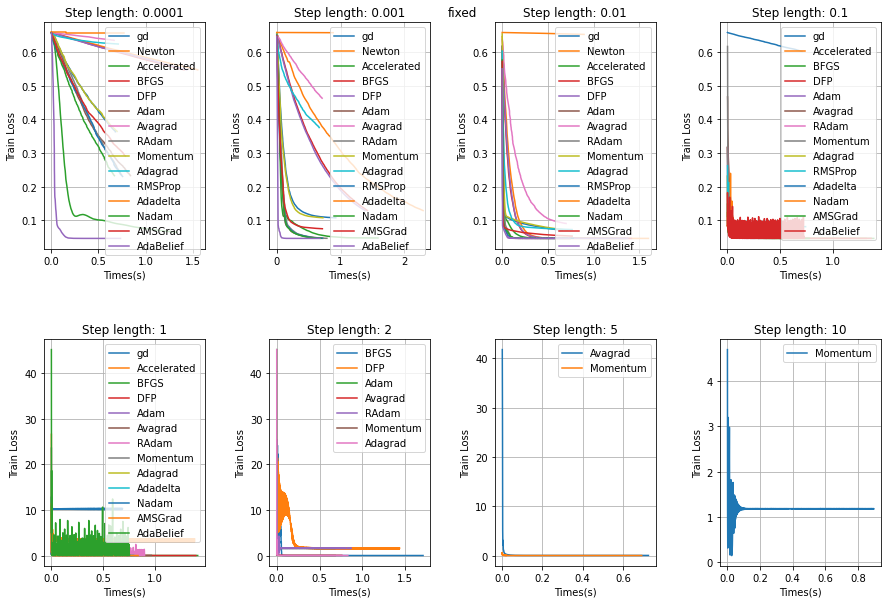
\includegraphics[width=10cm]{Thanh/fixed-lr-step-op_time.png}
		\caption{So sánh các thuật toán với phương pháp cố định step size}
	\end{figure}

	\begin{figure}
		\centering
		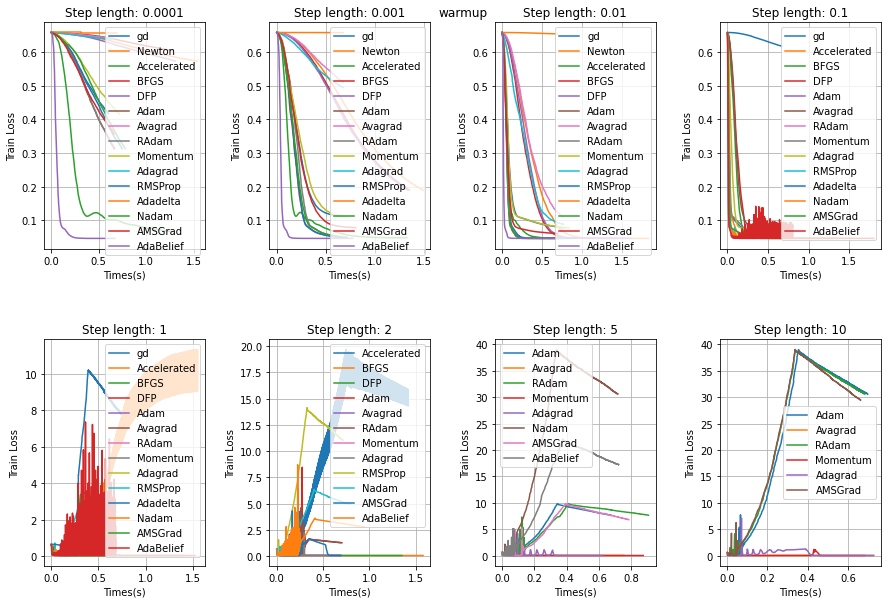
\includegraphics[width=10cm]{Thanh/warmup-lr-step-op_time.png}
		\caption{So sánh các thuật toán với phương pháp warmup step size}
	\end{figure}

	\begin{figure}
		\centering
		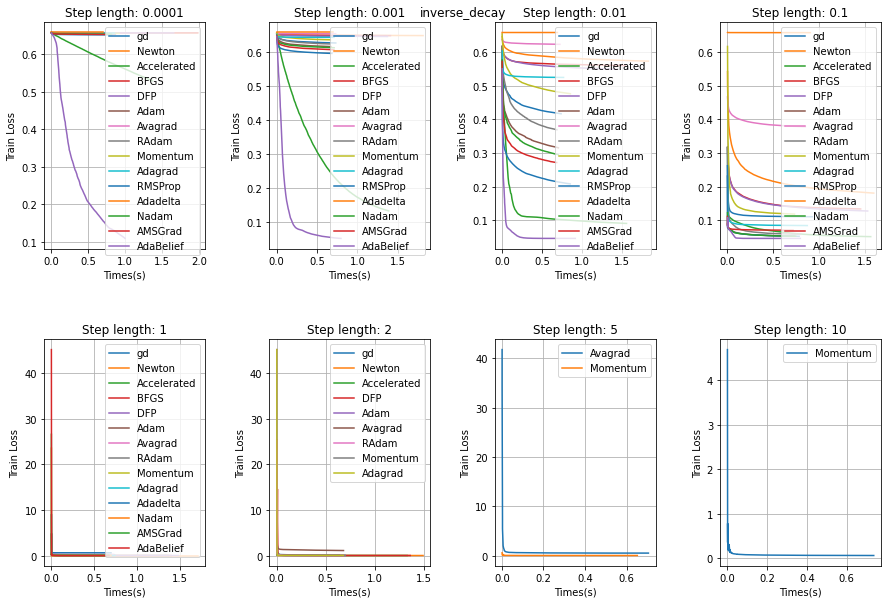
\includegraphics[width=10cm]{Thanh/inverse-lr-step-op_time.png}
		\caption{So sánh các thuật toán với phương pháp giảm step size dạng hyperbol}
	\end{figure}
\end{frame}

\begin{frame}{So sánh nhiều thuật toán}

	Thời gian đạt điều kiện hội tụ nhỏ nhất của từng thuật toán:
	

	Tập train (sự thay đổi loss tương đối nhỏ hơn $10^{-3}$ và chuẩn của vector gradient nhỏ hơn $10^{-4}$)
	Tập train (sự thay đổi loss tương đối nhỏ hơn $10^{-3}$ và chuẩn của vector gradient nhỏ hơn $10^{-3}$)

\end{frame}

\begin{frame}{So sánh nhiều thuật toán}

	\begin{table} [h!]
		\centering
		\resizebox{\linewidth}{!}{
		\begin{tabular}{ || c | c | c | c | c | c | c | c | c | c|| }
		\hline
		Thuật toán & Steps & Schedule & Step size & Loss & MAE & Inner steps & Time (s) & Grad norm & $R^2$ \\ [0.5 ex]
		\hline \hline
		GD & 304 & backtracking & 5 & 0.04698 & 0.1396 & 1218 & 0.7623 & 9.7491e-05 & 0.6548 \\ \hline
		Newton & 1 &  backtracking &  1 &  0.04642&  0.1396 & 1 &  0.004000&  1.7353e-16&  0.6589  \\ \hline
		Accelerated & 90 &  backtracking &  5 &  0.04678 &  0.1396 &  434 &  0.2740 &  8.9588e-05 &  0.6562 \\ \hline
		BFGS &28 &  backtracking &  10 &  0.04675 &  0.1399 &  82 &  0.07697 &  6.7362e-05 &  0.6565 \\ \hline
		DFP & 42 &  backtracking &  10 &  0.04690 &  0.1395 &  109 &  0.1965 &  9.5577e-05 &  0.6554 \\ \hline
		Adam & 55 &  backtracking &  5 &  0.04649 &  0.1394 &  383 &  0.1470 &  8.5136e-05 &  0.6584\\ \hline
		Avagrad & Null \\ \hline 
		RAdam &64 &  backtracking &  2 &  0.04643 &  0.1394 &  288 &  0.1457 &  5.9528e-05 &  0.6588 \\ \hline
		Momentum &  83 &  backtracking &  5 &  0.04685 &  0.1401 &  495 &  0.2240 &  9.9035e-05 &  0.6557 \\ \hline
		Adagrad & 223 &  backtracking &  2 &  0.0465 &  0.1392 &  629 &  0.5130 &  9.5012e-05 &  0.6579 \\ \hline
		RMSProp & 301 &  backtracking &  5 &  0.04644 &  0.1400 &  3130 &  0.9421 &  8.6495e-05 &  0.6588\\ \hline
		Adadelta & 525 &  backtracking &  2 &  0.04654 &  0.1398 &  12219 &  2.7243 &  9.9677e-05 &  0.6581\\ \hline
		Adamax & 65 &  backtracking &  5 &  0.04675 &  0.1403 &  413 &  0.1679 &  9.3636e-05 &  0.6565 \\ \hline
		Nadam & 77 &  backtracking &  5 &  0.04655 &  0.1394 &  611 &  0.2230 &  8.5295e-05 &  0.6580 \\ \hline
		AMSGrad & 76 &  backtracking &  10 &  0.04650 &  0.1393 &  586 &  0.2758 &  7.6637e-05 &  0.6583 \\ \hline
		AdaBelief & 41 &  backtracking &  5 &  0.04647 &  0.1393 &  294 &  0.1180 &  8.4853e-05 &  0.6585 \\ [1ex]
		\hline
		\end{tabular}
		}
		\caption{So sánh thời gian đạt điều kiện hội tụ trên tập train}
	\end{table}

\end{frame}

\begin{frame}{So sánh nhiều thuật toán}
	\begin{table} [h!]
		\centering
		\resizebox{\linewidth}{!}{
		\begin{tabular}{ || c | c | c | c | c | c | c | c | c | c|| }
		\hline
		Thuật toán & Steps & Schedule & Step size & Loss & MAE & Inner steps & Time (s) & Grad norm & $R^2$ \\ [0.5 ex]
		\hline \hline
		GD & 127 &  backtracking &  5 &  0.04840 &  0.1409 &  511 &  0.3030 &  0.0003 &  0.6282 \\ \hline
		Newton & 1 &  backtracking &  1 &  0.04750 &  0.1413 &  1 &  0.0040 &  0.0007 &  0.6351  \\ \hline
		Accelerated & 37 &  backtracking &  5 &  0.04891 &  0.1437 &  179 &  0.1119 &  0.0007 &  0.6243 \\ \hline
		BFGS &11 &  backtracking &  10 &  0.0492 &  0.1437 &  35 &  0.02998 &  0.0006 &  0.6214 \\ \hline
		DFP & 15 &  backtracking &  10 &  0.04915 &  0.1443 &  39 &  0.09148 &  0.0006 &  0.6225 \\ \hline
		Adam & 26 &  backtracking &  5 &  0.04797 &  0.1431 &  130 &  0.06000 &  0.0007 &  0.6315\\ \hline
		Avagrad & 129 &  fixed &  10 &  0.0689 &  0.1707 &  129 &  0.1146 &  0.0009 &  0.4704 \\ \hline 
		RAdam &31 &  backtracking &  1 &  0.04846 &  0.1421 &  66 &  0.06105 &  0.0003 &  0.6277 \\ \hline
		Momentum &  33 &  backtracking &  5 &  0.05161 &  0.1529 &  428 &  0.1320 &  0.0009 &  0.6036 \\ \hline
		Adagrad & 86 &  backtracking &  2 &  0.04813 &  0.1420 &  246 &  0.1910 &  0.0009 &  0.6303 \\ \hline
		RMSProp & 301 &  backtracking &  5 &  0.04761 &  0.1417 &  3130 &  0.9421 &  0.0006 &  0.6343\\ \hline
		Adadelta & 85 &  backtracking &  5 &  0.04833 &  0.1429 &  330 &  0.1920 &  0.0009 &  0.6288\\ \hline
		Adamax &29 &  backtracking &  1 &  0.05057 &  0.1492 &  319 &  0.1200 &  0.0009 &  0.6116 \\ \hline
		Nadam & 32 &  backtracking &  2 &  0.04873 &  0.1449 &  147 &  0.07400 &  0.0009 &  0.6257 \\ \hline
		AMSGrad & 20 &  backtracking &  5 &  0.05018 &  0.1434 &  150 &  0.057002 &  0.0006 &  0.6146 \\ \hline
		AdaBelief & 23 &  backtracking &  5 &  0.04848 &  0.1422 &  129 &  0.06500 &  0.0003 &  0.6276 \\ [1ex]
		\hline
		\end{tabular}
		}
		\caption{So sánh thời gian đạt điều kiện hội tụ trên tập validation}
	\end{table}

\end{frame}

\begin{frame}{So sánh nhiều thuật toán}

	\begin{table} [h!]
		\centering
		\resizebox{\linewidth}{!}{
		\begin{tabular}{ || c | c | c | c | c | c | c | c | c | c|| }
		\hline
		Thuật toán & Min loss & Schedule & Step size & MAE & Steps & Inner steps & Time (s) & Grad norm & $R^2$ \\ [0.5 ex]
		\hline \hline
		GD & 0.04642 &  backtracking &  5 &  0.1395 &  4999 &  19998 &  11.9320 &  5.9560e-06 &  0.6589 \\ \hline
		Newton & 0.04642 &  inverse decay &  2 &  0.1395 &  4285 &  4285 &  6.4144 &  1.1830e-05 &  0.6589  \\ \hline
		Accelerated & 0.04642 &  backtracking &  5 &  0.1396 &  4855 &  23379 &  16.02871 &  2.7890e-09 &  0.6589 \\ \hline
		BFGS &0.04642 &  warmup &  1 &  0.1396 &  3708 &  3708 &  6.1286 &  6.8517e-14 &  0.6589 \\ \hline
		DFP & 0.04642 &  warmup &  1 &  0.1396 &  4495 &  4495 &  6.3558 &  2.6095e-12 &  0.6589 \\ \hline
		Adam & 0.04642 &  backtracking &  0.001 &  0.1396 &  3664 &  33971 &  12.6386 &  5.4339e-11 &  0.6589\\ \hline
		Avagrad & 0.04972 &  backtracking &  10 &  0.1411 &  4999 &  5055 &  9.5528 &  0.0008 &  0.6347 \\ \hline 
		RAdam &0.04642 &  backtracking &  0.001 &  0.1396 &  3987 &  41786 &  14.8537 &  8.07073e-11 &  0.6589 \\ \hline
		Momentum &  0.04642 &  backtracking &  10 &  0.1396 &  4612 &  17849 &  9.9354 &  4.5472e-11 &  0.6589 \\ \hline
		Adagrad & 0.04642 &  backtracking &  1 &  0.1396 &  3986 &  8605 &  8.1345 &  1.2800e-10 &  0.6589 \\ \hline
		RMSProp & 0.04642 &  backtracking &  0.1 &  0.1396 &  4874 &  97153 &  26.7683 &  1.9558e-12 &  0.6589\\ \hline
		Adadelta & 0.04642 &  backtracking &  2 &  0.1396 &  4999 &  1231808 &  218.7172 &  1.6255e-05 &  0.6589\\ \hline
		Adamax &0.04642 &  backtracking &  0.01 &  0.13961 &  4104 &  75850 &  18.7867 &  2.2710e-11 &  0.6589 \\ \hline
		Nadam & 0.04642 &  backtracking &  0.01 &  0.1396 &  4882 &  107711 &  24.3817 &  5.6385e-11 &  0.6589 \\ \hline
		AMSGrad & 0.04642 &  warmup &  2 &  0.1396 &  4452 &  4452 &  3.5742 &  1.7151e-12 &  0.6589 \\ \hline
		AdaBelief & 0.04642 &  backtracking &  0.0001 &  0.1396 &  1794 &  19980 &  6.0632 &  3.2365e-11 &  0.6589 \\ [1ex]
		\hline
		\end{tabular}
		}
		\caption{So sánh thời gian đạt giá trị loss nhỏ nhất trên tập train}
	\end{table}

\end{frame}


\begin{frame}{So sánh nhiều thuật toán}

	\begin{table} [h!]
		\centering
		\resizebox{\linewidth}{!}{
		\begin{tabular}{ || c | c | c | c | c | c | c | c | c | c|| }
		\hline
		Thuật toán & Min loss & Schedule & Step size & MAE & Steps & Inner steps & Time (s) & Grad norm & $R^2$ \\ [0.5 ex]
		\hline \hline
		GD & 0.04720 &  cyclic &  1 &  0.1400 &  1778 &  1778 &  1.2055 &  0.0001 &  0.6374 \\ \hline
		Newton & 0.04733 &  fixed &  0.01 &  0.14063 &  1436 &  1436 &  2.2674 &  0.0009 &  0.6364  \\ \hline
		Accelerated & 0.04727 &  cyclic &  0.01 &  0.1405 &  1371 &  1371 &  1.9054 &  0.0007 &  0.6369\\ \hline
		BFGS &0.04729 &  warmup &  0.1 &  0.1405 &  328 &  328 &  0.4802 &  0.0002 &  0.6368 \\ \hline
		DFP & 0.04727 &  warmup &  1 &  0.1391 &  446 &  446 &  0.6439 &  0.0006 &  0.6369 \\ \hline
		Adam & 0.04730 &  fixed &  0.001 &  0.1409 &  1073 &  1073 &  0.7792 &  0.0004 &  0.6367\\ \hline
		Avagrad & 0.04958 &  backtracking &  10 &  0.1428 &  4999 &  5055 &  9.5528 &  0.001417 &  0.6192 \\ \hline 
		RAdam &0.04731 &  backtracking &  0.001 &  0.1410 &  1095 &  1095 &  2.2251 &  0.0005 &  0.6366 \\ \hline
		Momentum & 0.04732 &  backtracking &  10 &  0.1409 &  140 &  634 &  0.3140 &  0.0004 &  0.6365 \\ \hline
		Adagrad & 0.04735 &  fixed &  2 &  0.1410 &  648 &  648 &  0.5333 &  0.0007 &  0.6363 \\ \hline
		RMSProp & 0.04730 &  inverse decay &  1 &  0.1408 &  607 &  607 &  0.4155 &  0.0002 &  0.6367\\ \hline
		Adadelta & 0.04731 &  cyclic &  1 &  0.1408 &  4467 &  4467 &  3.0681 &  0.0002 &  0.6366\\ \hline
		Adamax &0.04732 &  backtracking &  5 &  0.1409 &  115 &  660 &  0.2840 &  0.0005 &  0.6365 \\ \hline
		Nadam & 0.04731 &  backtracking &  0.001 &  0.1409 &  1169 &  1169 &  1.9850 &  0.0005 &  0.6366 \\ \hline
		AMSGrad & 0.04734 &  fixed &  2 &  0.1411 &  468 &  468 &  0.3943 &  0.0007 &  0.6364 \\ \hline
		AdaBelief & 0.04735 &  inverse decay &  1 &  0.1406 &  203 &  203 &  0.1407 &  0.0002 &  0.6363 \\ [1ex]
		\hline
		\end{tabular}
		}
		\caption{So sánh thời gian đạt giá trị loss nhỏ nhất trên tập validation}
	\end{table}

\end{frame}

\begin{frame}[allowframebreaks]{Tài liệu tham khảo}
    \printbibliography
\end{frame}

\begin{frame}[allowframebreaks]{Phụ lục}
	\begin{enumerate}
		\item  Gradient Descent
		\begin{equation*}
			\begin{cases}g_t = \nabla f(w_{t-1}) \\ w_t = w_{t-1} - \alpha g_t\end{cases}
		\end{equation*}
		\item Momentum
		\begin{equation*}
			\begin{cases}m_0 = 0 \\ g_t = \nabla f(w_{t-1}) 
				\\ m_t = \beta_1 m_{t-1} + (1-\beta_1)g_t\\ w_t = w_{t-1} - \alpha m_t\end{cases}
		\end{equation*}
		\item Adagrad
		\begin{equation*}
			\begin{cases}v_0 = 0\\ g_t = \nabla f(w_{t-1}) \\ v_t = v_{t-1} + g_t^2 \\ w_t = w_{t-1} - \alpha \dfrac{g_t}{\sqrt{v_t} + \epsilon} \end{cases}
		\end{equation*}
		\item Adadelta
		\begin{equation*}
			\begin{cases}v_0 = 0\\d_0 = 0 \\ g_t = \nabla f(w_{t-1}) \\ v_t = \beta v_{t-1} + (1-\beta)g_t^2 \\ \Delta w = - \alpha \dfrac{\sqrt{d_{t-1} + \epsilon}g_t}{\sqrt{v_t + \epsilon}} \\ w_t = w_{t-1} + \Delta w \\ d_t = \beta d_{t-1} + (1 - \beta) \Delta w^2 \end{cases}
		\end{equation*}
		\item RMSProp
		\begin{equation*}
			\begin{cases}v_0 = 0\\ g_t = \nabla f(w_{t-1}) \\ v_t = \beta v_{t-1} + (1-\beta)g_t^2 \\ w_t = w_{t-1} - \alpha \dfrac{g_t}{\sqrt{v_t} + \epsilon} \end{cases}
		\end{equation*}
		\item Adam
		\begin{equation*}
			\begin{cases}m_0 = 0\\ v_0 = 0\\ g_t = \nabla f(w_{t-1}) \\ m_t = \beta_1 m_{t-1} + (1-\beta_1) g_t \\ v_t = \beta_2 v_{t-1} + (1-\beta_2)g_t^2 \\
				\hat{m}_t = \dfrac{m_t}{1 - \beta_1^t} \\ \hat{v}_t = \dfrac{v_t}{1 - \beta_2^t} \\ w_t = w_{t-1} - \alpha \dfrac{\hat{m}_t}{\sqrt{\hat{v}_t} + \epsilon} \end{cases}
		\end{equation*}
		\item Adamax
		\begin{equation*}
			\begin{cases}m_0 = 0\\ u_0 = 0 \\ g_t = \nabla f(w_{t-1}) \\ m_t = \beta_1 m_{t-1} + (1-\beta_1) g_t \\ u_t = \max(\beta_2 u_{t-1}, \lVert g_t \rVert_{\infty}) \\ w_t = w_{t-1} - \alpha \dfrac{m_t}{(1 - \beta_1^t)u_t + \epsilon}\end{cases}
		\end{equation*}
		\item AMSGrad
		\begin{equation*}
			\begin{cases}m_0 = 0\\ v_0 = 0\\ g_t = \nabla f(w_{t-1}) \\ m_t = \beta_1 m_{t-1} + (1-\beta_1) g_t \\ v_t = \beta_2 v_{t-1} + (1-\beta_2)g_t^2 \\ \hat{v}_t = \max(\hat{v}_{t-1}, v_t) \\ w_t = w_{t-1} - \alpha \dfrac{m_t}{\sqrt{\hat{v}_t} + \epsilon} \end{cases}
		\end{equation*}
		\item Nadam
		\begin{equation*}
			\begin{cases}m_0 = 0\\ v_0 = 0\\ g_t = \nabla f(w_{t-1}) \\ m_t = \beta_1 m_{t-1} + (1-\beta_1) g_t \\ v_t = \beta_2 v_{t-1} + (1-\beta_2)g_t^2 \\
				\hat{m}_t = \dfrac{m_t}{1 - \beta_1^t} \\ \hat{v}_t = \dfrac{v_t}{1 - \beta_2^t} \\ w_t = w_{t-1} -  \dfrac{\alpha}{\sqrt{\hat{v}_t} + \epsilon}\Bigg(\beta_1\hat{m}_t + \dfrac{1-\beta_1}{1-\beta_1^t}g_t\Bigg) \end{cases}
		\end{equation*}
		\item AdaBelief
		\begin{equation*}
			\begin{cases}m_0 = 0\\ s_0 = 0\\ g_t = \nabla f(w_{t-1}) \\ m_t = \beta_1 m_{t-1} + (1-\beta_1) g_t \\ s_t = \beta_2 s_{t-1} + (1-\beta_2)(g_t - m_t)^2 + \epsilon\\
				\hat{m}_t = \dfrac{m_t}{1 - \beta_1^t} \\ \hat{s}_t = \dfrac{s_t}{1 - \beta_2^t} \\ w_t = w_{t-1} - \alpha \dfrac{\hat{m}_t}{\sqrt{\hat{s}_t} + \epsilon} \end{cases}
		\end{equation*}
		\item Accelerated Gradient
		\begin{equation*}
			\begin{cases}v_t = w_{t-1} + \dfrac{t - 1}{t + 2} \big(w_{t-1} - w_{t-2} \big) \\
			w_{t+1} = v_t - \alpha \nabla f(v_t) \end{cases}
		\end{equation*}
		\item RAdam
		\begingroup
			\scalebox{0.8}{
				\begin{minipage}{1.2 \linewidth}
					\begin{algorithm}[H]
						\caption{Thuật toán RAdam}
						\hspace*{\algorithmicindent} \textbf{Input:} {độ dài bước $\lbrace \alpha_t \rbrace_{t=1}^{T}$, các hệ số $\beta_1, \beta_2$, $w_0$ khởi tạo, hàm mục tiêu $f(w)$} \\
						\hspace*{\algorithmicindent} \textbf{Output:} {$w$ đã được học}
						\begin{algorithmic}[1]
							\State{$m_0 \leftarrow 0$}
							\State{$v_0 \leftarrow 0$}
							\State{$\rho_{\infty} \leftarrow 2/(1-\beta_2)-1$}
							\For{$t=1$ to $T$}
								\State{$g_t \leftarrow \nabla f(w_{t-1})$}
								\State{$m_t \leftarrow \beta_1 m_{t-1} + (1 - \beta_1)g_t$}
								\State{$v_t \leftarrow \beta_2 v_{t-1} + (1 - \beta_2)g_t^2$}
								\State{$\widehat{m}_t \leftarrow m_t / (1 - \beta_1^t)$}
								\State{$\rho_t \leftarrow \rho_{\infty} - 2t\beta_2^t / (1 - \beta_2^t)$}
								\If {$\rho_t < 4$}
									\State{$\widehat{v}_t \leftarrow \sqrt{v_t / (1 - \beta_2^t)}$}
									\State{$r_t \leftarrow \sqrt{\frac{(\rho_t - 4)(\rho_t - 2)\rho_{\infty}}{(\rho_{\infty} - 4)(\rho_{\infty} - 2)\rho_t}}$}
									\State{$w_t \leftarrow w_{t-1} - \alpha r_t \widehat{m}_t / (\widehat{v}_t + \epsilon)$}
								\Else
									\State{$w_t \leftarrow w_{t-1} - \alpha \widehat{m}_t$}
								\EndIf
							\EndFor
							\State \Return $w_T$
						\end{algorithmic}
					\end{algorithm}
				\end{minipage}
			}
		\endgroup
		\item Avagrad
		\begin{equation*}
			\begin{cases} w_0 \in \mathbb{R}^d \\ m_0 = 0 \\ v_0 = 0 \\
			g_t = \nabla f(w_{t-1}) \\
			m_t = \beta_1 m_{t-1} + (1-\beta_1)g_t \\
			\eta_t = \dfrac{1}{\sqrt{v_{t-1}} + \epsilon} \\
			w_t = w_{t-1} - \alpha \dfrac{\eta_t}{\lVert \eta_t / \sqrt{d} \rVert_2} \odot m_t \\
			v_t = \beta_2 v_{t-1} + (1 - \beta_2) g_t^2\end{cases}
		\end{equation*}
		\item BFGS
		\begin{equation*}
			\begin{cases} \text{Khởi tạo } H_0 \\
			g_t = \nabla f(w_{t-1}) \\
			p_t = H_{t-1} g_t \\
			w_t = w_{t-1} - \alpha p_t \\
			s_t = w_t - w_{t-1} \\
			y_t = \nabla f(w_t) - \nabla f(w_{t-1}) \\
			H_t = \Bigg(I - \dfrac{s_t y_t^T}{y_t^T s_t} \Bigg)H_{t-1}\Bigg( I - \dfrac{y_t s_t^T}{y_t^T s_t} \Bigg) + \dfrac{s_t s_t^T}{y_t^T s_t}\end{cases}
		\end{equation*}
		\framebreak
		\item DFP
		\begin{equation*}
			\begin{cases} \text{Khởi tạo } H_0 \\
			g_t = \nabla f(w_{t-1}) \\
			p_t = H_{t-1} g_t \\
			w_t = w_{t-1} - \alpha p_t \\
			s_t = w_t - w_{t-1} \\
			y_t = \nabla f(w_t) - \nabla f(w_{t-1}) \\
			H_t = H_{t-1} - \dfrac{H_{t-1}y_t y_t^T H_{t-1}}{y_t^T H_{t-1} y_t} + \dfrac{s_t s_t^T}{y_t^T s_t}\end{cases}
		\end{equation*}
	\end{enumerate}
\end{frame}

\end{document}